% =====================================================================================
%  Section 4.7 — Are there other channels for safety?
%  Self-contained. Nothing to \input.
%
%  PREAMBLE (already in main.tex): graphicx, booktabs, multirow, threeparttable
%  ASSETS: figures/fig_rl_bracket.pdf, figures/fig_bon_correlation.pdf
%    Regenerate both:  PYTHONPATH=. python -m experiments.make_fig_channels
%
%  THE SUMMARY TABLE IS THE POINT OF THIS SECTION. Four negatives spread over several pages
%  read as a list of things that did not work; the same four with their tested scope stated
%  read as a bounded result. If space forces a cut, cut prose and keep Table 4.7.
%
%  EVERY NEGATIVE HERE IS SCOPED. Do not let any of them be restated as a general claim:
%  the RL result is about the reward design tested, best-of-N is about this policy and
%  benchmark, guided sampling is about an end-effector barrier, and the language result is
%  about the phrasing tested.
% =====================================================================================

\section{Are There Other Channels for Safety?}\label{sec:res:channels}

Four further mechanisms were tested and none replaced the shielded-imitation route. They are
reported together because a characterised negative bounds the claim of this work in a way a
positive result cannot, and because each fails for a different and identifiable reason.
Table~\ref{tab:negatives} summarises them; the subsections give the evidence.

\begin{table}[htbp]
\centering
\begin{threeparttable}
\caption[Mechanisms tested and rejected]{%
  Mechanisms tested and rejected, with the scope at which each negative is claimed. None is a
  general claim about its method class.}
\label{tab:negatives}
\footnotesize
\begin{tabular}{p{0.17\linewidth}p{0.24\linewidth}p{0.22\linewidth}p{0.27\linewidth}}
\toprule
\textbf{Mechanism} & \textbf{What was tested} & \textbf{Outcome} & \textbf{Scope of the negative} \\
\midrule
Scalar-reward RL
  & Flow-SDE GRPO on the action head, 4 configurations $\times$ 6 rounds, one scene
  & Either collapses to inaction or learns nothing; no setting does both
  & The reward design and budget tested. Not safe RL as a class; constrained-MDP and
    world-model methods supply richer signals \\
\addlinespace[3pt]
Language-expressed constraint
  & One safety clause appended to the instruction, $n=60$ per condition, level II
  & No safety change; 23\% slower, 11.7 points less successful
  & The single phrasing tested: generic, unnamed referent, manner adverbial \\
\addlinespace[3pt]
CBF-guided sampling
  & Barrier gradient injected into the flow integration, validated on a synthetic barrier
  & Never activates on real scenes; closest approach 0.231\,m against a 0.15\,m barrier
  & Guidance built on an \emph{end-effector} barrier. Untested with the full arm-link
    constraint set \\
\addlinespace[3pt]
Best-of-$N$ selection
  & $K \in \{4, 8\}$ candidates re-simulated per query, exact state rewind
  & No safe candidate on $\sim$60\% of queries; doubling $K$ buys 8.8 points
  & This policy and benchmark. The measurement it yields is reported as the result \\
\bottomrule
\end{tabular}
\begin{tablenotes}[flushleft]\footnotesize
\item Two further \emph{explanations}, as opposed to mechanisms, were also tested and rejected in
  Section~\ref{sec:res:mechanism}: observation aliasing and generative uncertainty.
\end{tablenotes}
\end{threeparttable}
\end{table}

\subsection*{Scalar-reward reinforcement learning}

Reinforcement learning was tried first, and its failure is what motivated the imitation approach
that the rest of this chapter evaluates. It is reported at length because the failure is
structural, and because four runs are needed to establish that.

The setup was flow-SDE GRPO on $\pi_{0.5}$'s flow-matching action head: the deterministic sampling
ODE is converted to an equivalent SDE so that log-probabilities exist and a policy gradient can be
taken. A LoRA adapter on the action head received gradients with the backbone frozen, matching the
trainable surface used for distillation in Section~\ref{sec:res:internalise}, so the comparison
between the two learning signals is not confounded by capacity. Rollouts used the CPS sampler at
noise 0.7 with ten denoising steps and clipping 0.2, on one level-II scene, with $K = 8$ rollouts
per group over six rounds. The reward combined success, direct collision, CBF activation rate and
progress terms.

\begin{figure}[htbp]
  \centering
  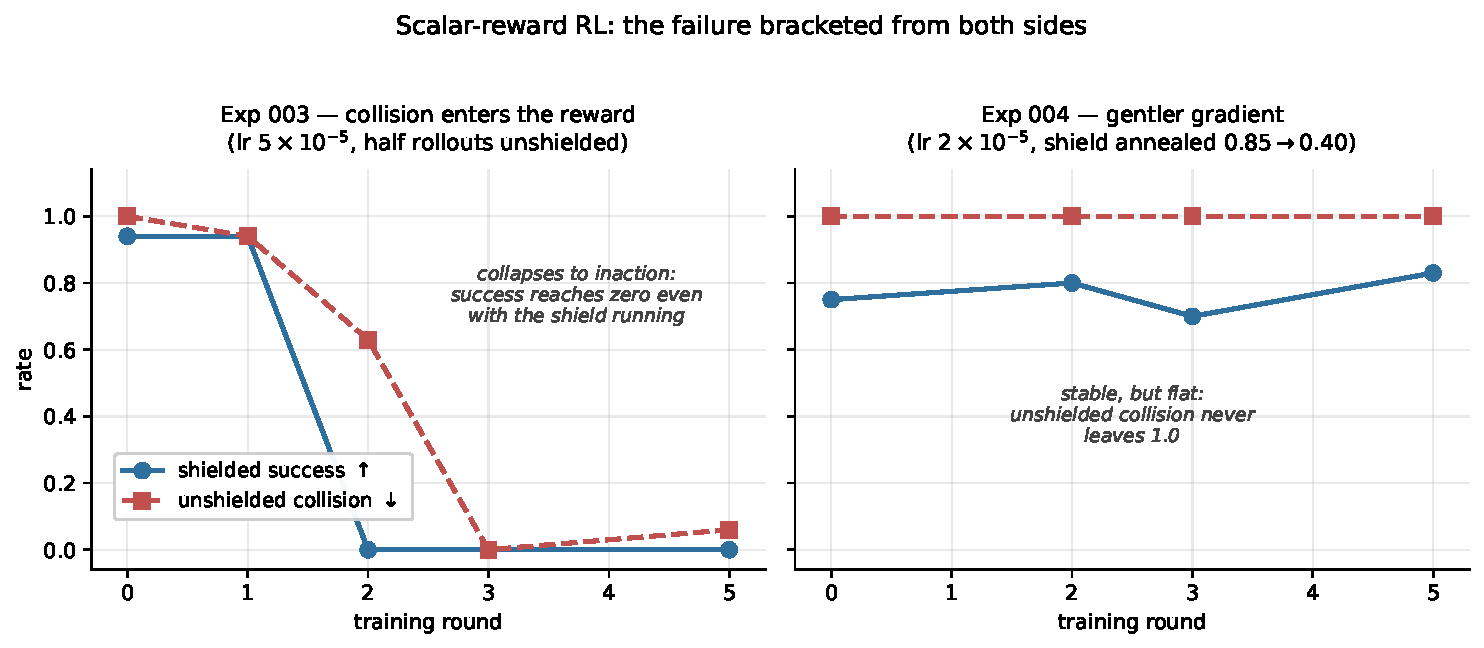
\includegraphics[width=\linewidth]{figures/fig_rl_bracket.pdf}
  \caption[Scalar-reward RL bracketed from both sides]{%
    The two informative configurations. \textbf{Left:} admitting real collisions to the reward
    moves the policy, and it collapses --- success reaches zero \emph{in the shielded condition
    too}, which the shield alone cannot cause, so the policy has found the trivial zero-collision
    optimum of doing nothing. \textbf{Right:} a lower learning rate with an annealed shield fixes
    the collapse and learns nothing, with unshielded collision pinned at 1.0 for six rounds.
    Neither panel alone is an argument; together they are the two sides of one knob.}
  \label{fig:rl_bracket}
\end{figure}

\paragraph{Too weak.}
With the shield active on every rollout, collisions never enter the reward directly --- the shield
prevents them --- so the only safety signal is the CBF activation penalty. Raising the learning
rate to $5 \times 10^{-5}$ and the activation weight to 1.5 left the policy flat.

\paragraph{Too strong.}
Running half of each group's rollouts unshielded puts real collisions into the reward, widening the
within-group spread to roughly $\Delta = 1.0$. The safety metric improved immediately and the task
collapsed with it. Two causes compound: the adapter diverged, since the mixed reward is far higher
variance than the flat one at the same learning rate; and the collision penalty punishes progress,
because in these scenes the obstacle lies between the gripper and the goal, so nearly all forward
motion collides early in training.

\paragraph{What the bracket establishes.}
The only configuration that moved the policy's behaviour collapsed it; every configuration stable
enough to preserve the task learned no avoidance. That is not a gap between two tuned settings but
the two sides of a single one. The learning signal and the destabilising signal are the same knob,
for two compounding reasons. A single scalar episode reward gives no per-step spatial credit, so
the policy cannot separate ``detour around the obstacle'' from ``stop moving toward the goal'' when
the obstacle lies on the path to the goal. And in a flow-matching policy, exploration \emph{is}
sampling noise, which is also what degrades the actions being evaluated.

This is precisely what the shield supplies and the reward does not. The barrier already computes
the correct action at every step it intervenes, in the same space the policy emits, so the credit
assignment the reward could not infer is simply given.

\subsection*{Safety expressed in language}

Every mechanism examined so far acts on the action. A vision-language-action model exposes a
channel none of them use, and one a classical controller does not possess at all --- the
instruction itself.

The experiment is minimal by design: the same checkpoint, seed, held-out initial states and
evaluation code for both conditions, differing only in a clause appended to the instruction. Twelve
level-II scenes at five initial states each give $n = 60$ per condition; level II was chosen
because collisions concentrate there.

\begin{quote}\small
\textbf{plain:} \texttt{pick up the black bowl between the plate and the ramekin and place it on
the plate}\\[3pt]
\textbf{safety:} \texttt{\dots{} and place it on the plate, being careful not to touch or knock
over any other objects}
\end{quote}

The suffix is reproduced verbatim because a negative about language is only as strong as the
language tested. The phrasing is generic: it names no object, gives no spatial reference, and
states the constraint as a manner adverbial rather than a prohibition. Each is a design choice that
could plausibly matter, and none was varied.

\begin{table}[htbp]
\centering
\caption{Effect of appending a safety clause to the instruction. $n = 60$ per condition, twelve
  level-II scenes, Wilson 95\% intervals.}
\label{tab:language}
\begin{tabular}{lccc}
\toprule
\textbf{Condition} & \textbf{TSR (95\% CI)} & \textbf{Collision (95\% CI)} & \textbf{ETS} \\
\midrule
Plain instruction       & 66.7\% [54.1, 77.3] & 70.0\% [57.5, 80.1] & 132.4 \\
Safety clause appended  & 55.0\% [42.5, 66.9] & 68.3\% [55.8, 78.7] & 162.4 \\
\bottomrule
\end{tabular}
\end{table}

Collisions fall by 1.7 percentage points, with almost coincident intervals. But the policy is not
ignoring the text: execution time rises 23\% and success falls 11.7 points, while the per-body
attribution shows no meaningful redistribution. The policy responds to the safety clause by acting
more slowly and completing fewer tasks, without touching anything less often.

The natural reading is that safety language elicits a general behavioural prior --- hesitancy,
reduced speed --- rather than a grounded avoidance behaviour. The model has learned that
safety-flavoured instructions correspond to cautious-looking motion, and that association is not
connected to the geometry of the scene. It produces the appearance of caution without its
substance. The distinction matters: it separates ``the model ignores safety language'' from ``the
model responds to safety language but does not ground it'', and only the second says anything about
what such a channel would need.

\subsection*{CBF-guided sampling}

The shield corrects an action after the policy has produced it. A flow-matching policy offers an
earlier point of intervention: the action is generated by integrating an ODE over several denoising
steps, so a barrier gradient can be injected \emph{into} that integration, steering generation
toward safe actions rather than projecting unsafe ones afterwards.

The implementation was validated before deployment, because two sign and scheduling conventions
produce plausible-looking but incorrect behaviour. On a synthetic barrier with a known closed-form
projection, $\lambda = 1$ reproduces the projection endpoint exactly.

On real scenes it never fired. Across level-II episodes the end-effector's closest approach to the
obstacle was 0.231\,m against a barrier radius of 0.15\,m --- the guidance term was identically
zero for the entire rollout --- while those same episodes collided. The reason is the one
Section~\ref{sec:res:scope} identifies: the barrier is a function of the end-effector, and the
contacts that occur are made by the arm links. Guidance inherits the scope of the barrier it steers
by, so steering generation cannot reach a failure the barrier cannot see. This is a scope-limited
negative, and it would be worth revisiting on a barrier carrying the full arm-link constraint set.

\subsection*{Best-of-$N$ selection, and what it measured instead}

If safety varied across the actions a policy might sample from a given state, it could be obtained
by rejection: draw $K$ candidate action chunks, simulate each, execute the safest. The sampler must
be stochastic for candidates to differ, so the matched control is $K = 1$ at the same noise level
rather than the deterministic policy used elsewhere in this chapter. Making the measurement
trustworthy required the simulator to be rewound exactly between candidates; snapshot and restore
were verified to machine precision before any result was recorded.

\begin{figure}[htbp]
  \centering
  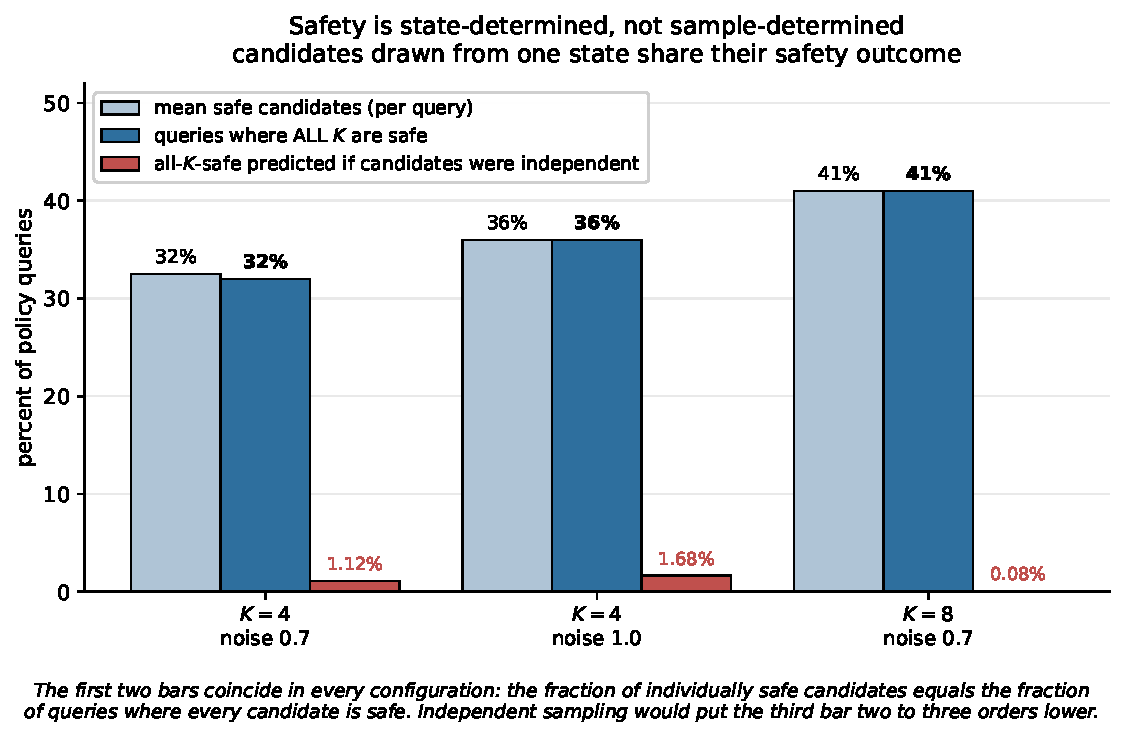
\includegraphics[width=0.82\linewidth]{figures/fig_bon_correlation.pdf}
  \caption[Within-state safety correlation in a VLA policy]{%
    Why rejection sampling cannot help here. In every configuration the fraction of individually
    safe candidates coincides with the fraction of queries in which \emph{all} $K$ are safe, so a
    query is $0$-of-$K$ or all-of-$K$ safe and almost never in between. Independent sampling would
    make the all-$K$-safe rate two to three orders of magnitude smaller (right-hand bars).}
  \label{fig:bon}
\end{figure}

As a method this is negative: on roughly 60\% of queries no candidate was safe, and buying more
candidates barely moved it --- doubling $K$ from four to eight recovered 8.8 percentage points for
twice the compute, and raising the noise recovered 3.7.

The measurement underneath it is the more interesting result. The mean safe fraction and the
all-$K$-safe fraction coincide in all three configurations. Were the candidates independent draws,
the all-$K$-safe rate would be $p^{K}$: 1.1\% at $K = 4$ and 0.08\% at $K = 8$, against observed
values of 32\% and 41\%. The policy's samples from a given state are therefore near-perfectly
correlated in their safety outcome.

Safety in this policy is consequently \textbf{state-determined rather than sample-determined}, at
least on this benchmark. Once a state is reached the outcome is largely fixed, and no amount of
choosing among actions recovers it --- the leverage lies in not reaching the state. This also
explains a result that would otherwise look inconsistent: episode-level filtering worked
(Section~\ref{sec:res:mechanism}) while action-level selection cannot, because episode-level
selection chooses between trajectories that reached \emph{different states}, which is the axis
along which variation actually exists.

The correlation measurement is offered here as the contribution rather than the selection method.
It is, as far as this work is aware, the first measurement of candidate-level safety correlation in
a vision-language-action policy, and it is the sharpest available statement of the reachability
theme running through Sections~\ref{sec:res:scope}, \ref{sec:res:mechanism} and the discussion that
follows.
